
%%%%%%%%%%%%%%%%%%%%%%%%%%%%%%%%%%%%%%%%%%%%%%%%%%%%%%%%%%%%%
%%%%%%%%%%%%%%%%%%%%%%%%%%%%%%%%%%%%%%%%%%%%%%%%%%%%%%%%%%%%%
%
%  %%%%%%%  %    %  %%%%%%  %%%%%%  %%%%%%%  %%%%%%%  %%%%%
%  %        %    %  %    %  %     %    %     %        %    %
%  %        %    %  %%%%%%  %     %    %     %        %    %
%  %        %%%%%%  %    %  %%%%%%     %     %%%%%    %%%%%
%  %        %    %  %    %  %          %     %        %    %
%  %%%%%%%  %    %  %    %  %          %     %%%%%%%  %     %
%
%%%%%%%%%%%%%%%%%%%%%%%%%%%%%%%%%%%%%%%%%%%%%%%%%%%%%%%%%%%%%
%%%%%%%%%%%%%%%%%%%%%%%%%%%%%%%%%%%%%%%%%%%%%%%%%%%%%%%%%%%%%

\chapter{Functors Associated to Maps}
\label{sec:maps}

\begin{quote}
{\em``Qui s\`eme le foncteur r\'ecolte la structure.''}\footnote{``Who sows the functor reaps the structure.''}
\begin{flushright} --- Bourbaki \end{flushright}
\end{quote}

Since sheaves and cosheaves as defined here assign data to open sets, maps between spaces should only make reference to open sets. In Section~\ref{subsec:six_ops} we briefly introduced how to pushforward or pullback a sheaf along a map between spaces. In the case where our spaces are partially ordered sets endowed with the Alexandrov topology, it suffices to work directly with points since they are in bijection with a basis for the topology. However, playing these perspectives off of each other adds depth to the theory. In particular, by restricting our attention to these spaces, and using Kan extensions, we define the basic functors on (co)sheaves without making use of (co)sheafification. Pedagogically this is advantageous because the operation of sheafification tends to obfuscate the underlying ideas of sheaf theory. The lack of an explicit cosheafification process has historically been a stumbling block for the theory.

Recall that the definition of a continuous map $f:X\to Y$ says that the inverse image of an open set of $Y$ is an open set of $X$. This observation can be expressed by saying that we have a functor
\[
\mathring{f}:\Open(Y)\to\Open(X) \qquad U\subseteq Y \rightsquigarrow f^{-1}(U)\subseteq X.
\]
By formality, we also have a functor from the corresponding opposite categories
\[
\mathring{f}:\Open(Y)^{op}\to\Open(X)^{op}.
\]
We have purposely suppressed the $op$ superscript on $\mathring{f}$ for legibility. Now suppose we are given a pre-sheaf $G$ on $X$, then we get a naturally associated pre-sheaf on $Y$ by observing that the diagram
\[
\xymatrix{\Open(X)^{op} \ar[r]^-G & \dat \\
\Open(Y)^{op} \ar[u]^{\mathring{f}} \ar@{-->}[ru] & }
\]
has a natural completion given by pre-composition. 

\begin{defn}[Pushforward Sheaf and Cosheaf]\index{sheaf!pushforward}\index{cosheaf!pushforward}\index{direct image}
	Suppose $f:X\to Y$ is a continuous map of spaces, $G$ and $\hG$ a pre-sheaf and pre-cosheaf respectively, then define the \textbf{pushforward} or \textbf{direct image} pre-sheaf and pre-cosheaf via $f_*G(U):=G(f^{-1}(U))$ and $f_*\hG(U):=\hG(f^{-1}(U))$. Because $f^{-1}$ commutes with unions, we get that if $G$ or $\hG$ is a sheaf or cosheaf, then so is the pushforward. Moreover, this operation is functorial with respect to maps between (co)sheaves, so we get functors
	\[
	f_*:\Shv(X;\dat) \to \Shv(Y;\dat) \qquad f_*:\Coshv(X;\dat)\to\Coshv(Y;\dat).
	\]
\end{defn} 

There is also a pullback functor associated to a continuous map $f:X\to Y$, but it's construction is less obvious. Namely, if $G$ is a pre-sheaf on $Y$, then there is no clear way to define a pre-sheaf on $X$ because for an open set on $X$, $f(U)$ may not be open. The solution usually used is to take a system of approximations of $f(U)$ by open sets and to define the pullback sheaf as the limit of these approximations.
\[
	f^*G(U):=\varinjlim_{V\supset f(U)} F(V).
\]

Thinking categorically, the problem of ``approximation'' has been encountered before. Namely, how can we complete the following diagram?
\[
\xymatrix{\Open(Y)^{op} \ar[r]^-G \ar[d]_{\mathring{f}} & \dat \\
\Open(X)^{op} \ar@{-->}[ru]_? & }
\]
Again, by assuming that $\dat$ has sufficient colimits, we can could fill in the diagram by taking the left Kan extension of $G$ along $\mathring{f}$ and that will yield the candidate formula for the pullback just presented. Unfortunately, this definition for the pullback of a sheaf does not always define a sheaf. In sheaf theory over general spaces, this defect is circumvented by sheafification, as in Section~\ref{subsec:six_ops}. Fortunately, for the Alexandrov topology, this circumvention is unnecessary.

\section{Maps of Posets and Associated Functors}
\label{subsec:map_functors}

As already noted, sheaves and cosheaves on posets are easier to manipulate. The functors associated to a map of posets are explicitly defined without extra processing. Since posets can be made into a topological space the functors which exist for sheaves on general spaces can be studied here is a more tightly controlled laboratory. Moreover, since Alexandrov spaces have extra symmetries new functors not normally encountered exist here. 

\begin{defn}[Map of Posets]\index{poset!maps}
	Suppose $(X,\leq_X)$ and $(Y,\leq_Y)$ are posets. A map of posets is a map of sets $f:X\to Y$ that is order-preserving, i.e. if $x\leq_X x'$ then $f(x)\leq_Y f(x')$. Alternatively, since a poset can be viewed as a category, a map of posets is just a functor. When it is clear from context we will abbreviate $(X, \leq_X)$ by just $X$.
\end{defn}

\begin{rmk}[Notation and Cell Complexes]\label{rmk:cell_notation}
	In our effort to treat posets as spaces, we have used $X$ and $Y$ to denote partially ordered sets equipped with the Alexandrov topology. This might cause confusion since our canonical example of a poset will be the indexing poset of a cell complex $(X,P_X)$. Note that cell complexes consist of a pair of spaces, one is $X$, the Hausdorff space that is partitioned into pieces $X_{\sigma}$, the other is $P_X$, the poset of labels $\sigma$. From here on out we will work primarily with the poset $P_X$ as this is the combinatorial approximation to $X$. 
Thus, keeping in line with Shepard~\cite{shepard}, we change our notation from $(X,P_X)$ to $(|X|,X)$. Thus we have the following dictionary:
\begin{center}
\begin{tabular}{c |  c  c}
	 Dictionary & Old Notation & New Notation \\
	\hline
	Underlying Hausdorff Space & $X$ & $|X|$ \\
	Underlying Alexandrov Space & $P_X$ & $X$ \\
	Set of Points in a ``Cell'' & $X_{\sigma}$ & $|\sigma|$ \\
	``Cell'' viewed as a point & $\sigma$ & $\sigma$ \\
	Cellular Sheaf & $F:P_X\to\dat$ & $F:X\to\dat$
\end{tabular}
\end{center}
\end{rmk}

\subsection{Pullback or Inverse Image}
\label{subsubsec:pullback}

Recall that a sheaf on a poset $(Y,\leq_Y)$ is a functor $G:Y\to\dat$.  Similarly, a cosheaf is a functor $\hF:Y^{op}\to\dat$. For both structures the pull-back functor $f^*$ is easily described. It is the obvious pre-composition that completes the following diagram.
\[
\xymatrix{Y \ar[r]^-G & \dat \\
X \ar[u]^{f} \ar@{-->}[ru] & }
\]

\begin{defn}[Pullback for Poset Maps]\index{pullback!of a sheaf over a poset}
	Given a sheaf $G$ on $Y$ and a map of posets $f:X\to Y$, we can define the \textbf{pullback} or \textbf{inverse image} sheaf $f^*G$ on $X$ as follows:
	\begin{itemize}
		\item $f^*G(x)=G(f(x))$
		\item If $x\leq x'$, then let $\rho^{f^*G}_{x',x}=\rho^G_{f(x'),f(x)}$
		\item If $\eta: G\to H$ is a morphism in $\Shv(Y)$, i.e. a natural transformation of diagrams over $Y$, then $f^*\eta: f^*G\to f^*H$ is a morphism in $\Shv(X)$ defined by declaring $f^*\eta(x):f^*G(x)\to f^*H(x)$ to be equal to $\eta(f(x)):G(f(x))\to H(f(x))$.
	\end{itemize}
	
	The same definition and arguments go through for a cosheaf on $Y$ with suitable modification, i.e $r^{f^*G}_{x,x'}=r^G_{f(x),f(x')}$. Thus, we get functors
	\[
	f^*:\Shv(Y;\dat) \to \Shv(X;\dat) \qquad f^*:\Coshv(Y;\dat)\to\Coshv(X;\dat).
	\] 
\end{defn}

The definition of the pullback seems almost too good to be true, but one can check that the pre-sheaf description we outlined earlier agrees with this definition. Observe that if one applies that definition then
\[
	f^*F(U_x):=\varinjlim_{V \supset f(U_x)} F(V) \cong F(V_{f(x)})=F(f(x)),
\]
where we have used the fact that the smallest open set containing $f(U_x)=f(\{x' | x\leq x'\})$ is $V_{f(x)}=\{y|f(x)\leq y\}$.

\begin{ex}[Constant Sheaf and Cosheaf]\index{sheaf!constant sheaf!pullback from a point}
 Consider the constant map $p:X\to\star$. A sheaf $G$ on $\star$ consists of a single vector space $W$ and the identity morphism so we'll just call $G$ by the name $W$. We define the constant sheaf on $X$ with value $W$ to be $W_X:=p^*W$. One sees that it is a sheaf that assigns $W$ to every cell with all the restriction maps being the identity. Similarly, the constant cosheaf with value $W$ is $\hat{W}_X:=p^* W$.
\end{ex}

\subsection{Application: Subdivision}
\label{subsubsec:subdivide}
In the case where the poset is the face relation of a cell complex certain natural maps present themselves, such as subdivision.
	
\begin{defn}[\cite{shepard} 1.5, p.29]\index{subdivision}\index{cell complex!subdivision}
 A \textbf{subdivision} of a cell complex $X$ is a cell complex $X'$ with $|X'|=|X|$ and where every cell of $X$ is a union of cells of $X'$.
\end{defn}

Untangling the definition a bit we see that if $\sigma$ is a cell of $X$, then there is a collection of cells $\{\sigma_i'\}$ such that $\cup_i |\sigma_i'|=|\sigma|$. As such, we can define a surjective map of posets $s:X'\to X$ defined by making $s(\sigma')=\sigma$ if $|\sigma'|\subseteq |\sigma|$.

\begin{clm}
 Subdivision of a cell complex $X$ induces an order preserving map $s:X'\to X$ of the corresponding face-relation posets.
\end{clm}
\begin{proof}
 The ordering on $X'$ is given by the face relation. Suppose $\sigma'\leq \tau'$, then either $s(\sigma')=s(\tau')$ or not. If not, then $\sigma'$ and $\tau'$ belong to the subdivision of two cells $\sigma\leq \tau$.
\end{proof}

We are going to use this fact to define the subdivision of a sheaf in a cleaner manner than is found in~\cite{shepard}.

\begin{defn}\index{subdivision!of a cellular sheaf}\index{sheaf!cellular!subdivision}
 Suppose $F$ is a sheaf on $X$ and $s:X'\to X$ is a subdivision of $X$, then we define the subdivided sheaf $F':=s^*F$.
\end{defn}

\subsection{Pushforward or Direct Image}
\label{subsubsec:pushforward}

By adopting a point-theoretic picture rather than an open set-theoretic picture of sheaves and cosheaves over posets, we got an easy definition for the pullback functor. In the introduction we outlined a general definition for the pushforward functor $f_*$ on sheaves and cosheaves on an arbitrary topological space. Interestingly enough, although $f_*$ had a simple description using open sets, the point-level description requires thought.

\begin{defn}[Pushforward for Poset Maps]\index{sheaf!pushforward}\index{cosheaf!pushforward}\index{direct image}

	 Given a sheaf $F$ on $X$ and a map of posets $f:X\to Y$ we can define a sheaf on $Y$ as follows:
	\begin{itemize}
	 \item The \textbf{pushforward} of a sheaf is the right Kan extension of $F$ along $f$, i.e. $\Ran_f F$. \[f_*F(y)=\varprojlim_{f(x)\geq y} F(x)\]
	 \item Suppose $y\leq y'$, then $\{x|f(x)\geq y'\}\subseteq \{x|f(x)\geq y\}$. Any limit over the bigger set defines a cone over the smaller set by restriction, thus the universal property of limits guarantees the existence of a unique map $f_*F(y)\to f_*F(y')$ that we will call $\rho^{f_*F}_{y',y}$.
	 \item Suppose $\eta:F\to G$ is a map of sheaves, i.e. a natural transformation of diagrams over $X$. Then for any sub-poset $U$ of $X$, post-composing the limit over $U$ of $F$ with the arrows in the natural transformation defines a cone over $G$ restricted to $U$. By the universal property of limits there must be an induced map. $$\varprojlim_{x\in U} F \to \varprojlim_{x\in U} G$$
	\end{itemize}
	
	For cosheaves, the dual arguments go through with the slight modification that we use the left Kan extension along $f^{op}:X^{op}\to Y^{op}$.
	\[f_*\hF(y):= \varinjlim_{f(x)\geq y}\hF(x).\]
	Since both of these constructions are functorial, we have redefined two functors:
	\[
	f_*:\Shv(X;\dat) \to \Shv(Y;\dat) \qquad f_*:\Coshv(X;\dat)\to\Coshv(Y;\dat)
	\]
\end{defn}

\begin{ex}[Global Sections]\index{global sections!pushforward to a point}\index{pushforward to a point}
This functor is extremely useful as it gives us a way of defining the global sections of a sheaf or a cosheaf. For the constant map $p:X\to \star$ we offer the following definitions:
\[
	p_* F(\star)\cong F(X) = \Gamma(X;F) = H^0(X;F) \qquad p_*\hF(\star) \cong \hF(X) = \Gamma(X;\hF) = H_0(X;\hF)
\]
In Section \ref{sec:derived} we will use this definition as the prototype for defining ``higher'' pushforward or direct image functors.
\end{ex}

\subsection{$f_{\dd}$, Pushforwards and Closed Sets}
\label{subsubsec:closed_push}

One of the advantages of describing the standard functors of sheaf theory in the setting of posets is the presence of extra symmetries. Abstract definitions lend themselves to being dualized. In particular, in our point-theoretic definition of the pushforward we made use of Kan extensions, which come in two variants: left and right. In this section we consider the other variant and give a topological explanation for its origin.

\begin{rmk}[Caveat]\index{f@$f_{\dd}$ notation}
	The functor $f_{\dd}$ defined below is the left adjoint to $f^*$ (for cosheaves it will be the right adjoint). There seems to be a strong trend to call the left adjoint of $f^*$ by a different name: $f_!$. According to Joel Friedman (\cite{friedman} p. 22) the tradition goes back to Grothendieck in~\cite{sga4.1} SGA Expos\'e I, Proposition 5.1. The same notation is used by Ladkani~\cite{sl-dereq}, Lurie, Beilinson, Bernstein and others.

	This is unfortunate, since the notation $f_!$ is perhaps even more firmly established for the pushforward with compact supports functor used in classical sheaf theory. The reason seems to be that for general sheaves, there is no left adjoint to $f^*$, so it would be clear from context which was meant. However, for cellular sheaves, both functors exist and are useful.
\end{rmk}

\begin{defn}[Pushforward with Open Supports]\index{pushforward with open supports $f_{\dd}$}\index{sheaf!pushforward $f_{\dd}$}
 Given a sheaf $F$ on $X$ and a map of posets $f:X\to Y$ we can define a sheaf on $Y$ as follows:
\begin{itemize}
 \item The \textbf{pushforward with open supports} of a sheaf is the left Kan extension of $F$ along $f$, i.e. $\Lan_f F$. \[f_{\dd}F(y)=\varinjlim_{f(x)\leq y} F(x)\]
 \item If $y\leq y'$, then $\{x|f(x)\leq y\}\subseteq\{x|f(x)\leq y'\}$ and since any colimit over the bigger set defines a cocone over the smaller set by restriction, we get a unique map $\rho^{f_{\dd}F}_{y',y}:f_{\dd}F(y)\to f_{\dd}F(y')$.
 \item If we have a map of sheaves $\eta:F\to G$, then pre-composing the arrows for $\colim G$ with $\eta$ defines a co-cone over $F$. By universal properties we get an induced map \[\varinjlim_{x\in V} F\to \varinjlim_{x\in V} G.\]
\end{itemize}

Dually, for cosheaves we use the right Kan extension along $f^{op}$.
\[f_{\dd}\hF(y):= \varprojlim_{f(x)\leq y}\hF(x)\]
Both of these constructions are functorial and thus we have defined two functors:
\[
f_{\dd}:\Shv(X;\dat) \to \Shv(Y;\dat) \qquad f_{\dd}:\Coshv(X;\dat)\to\Coshv(Y;\dat)
\]
\end{defn}

This functor appears to be quite unusual, despite its naturality from the categorical perspective. To explain its topological origin, we revisit some of the original ideas of Alexandrov.

When Alexandrov first defined his topology he did two things differently:
\begin{enumerate}
	\item He only defined the topology for \emph{finite} posets.
	\item He defined the \emph{closed} sets to have the property that if $x\in V$ and $x'\leq x$, then $x'\in V$.
\end{enumerate}
\index{cosheaf!on closed sets}\index{sheaf!on closed sets}
Let us repeat the initial analysis of sheaves and diagrams indexed over posets, where we now put closed sets on equal footing with open sets. Observe that as before we have an inclusion functor:
\[
 j:(X,\leq) \to \Closed(X) \qquad x \rightsquigarrow \bar{x}:=\{x'| x'\leq x\}
\]
Consequently, we have a similar diagram for a functor $F:X\to\dat$ as before.
\[
	\xymatrix{X \ar[r]^F \ar[d]_{j} & \dat \\
	\Closed(X) \ar@{.>}[ur]_{?} & }
\]

If we choose the left Kan extension, we'd like to say the extended functor is a cosheaf on closed sets, i.e. use the definition of a cosheaf but replace open sets with closed sets. Unfortunately, this concept is not well defined for general topological spaces because the arbitrary union (colimit) of closed sets is not always closed. For Alexandrov spaces this property does hold and this illustrates one of the extra symmetries this theory possesses.

However, in order for the Kan extension to take a diagram and make it into a cosheaf, we need to know whether the image of the inclusion functor defines a basis for the closed sets. In Example \ref{ex:closed_gen} we showed that this is not always the case. The topology generated by the image of this functor is called the \textbf{specialization} topology and it suffers from certain technical deficiencies. In particular, order-preserving maps are not necessarily continuous in this topology, thus it fails to give a functorial theory. Fortunately, for finite posets these topologies agree and we can talk about cosheaves on closed sets without any trouble.

We now can give a topological explanation for the existence of the functor $f_{\dd}$. It is the functor analogous to ordinary pushforward where we have adopted closed sets as the indexing category for cosheaves and sheaves. If $f:X\to Y$ is a map of posets, then $f^c$ is the induced map between closed sets. The dagger pushforward is then the obvious completion of the diagram.
\[
\xymatrix{\Closed(X) \ar[r]^-F & \dat \\
\Closed(Y) \ar[u]^{f^c} \ar@{-->}[ru]_{f_{\dd}F} & }
\]

In Section \ref{subsec:sheaf_homology} this functor provides the foundation for defining \textbf{sheaf homology} and \textbf{cosheaf cohomology} --- theories that don't exist for general spaces.

\subsection{$f_!$: Pushforward with Compact Supports on Cell Complexes}
\label{subsubsec:shriek}

The three functors $f^*,f_*$ and $f_{\dagger}$ induced by a map of posets are well defined for any poset and any diagram. However, when Shepard wrote his thesis the only posets that he considered were posets coming from cell complexes. By working in this smaller class and imitating the theory of constructible sheaves, Shepard described another functor that is not defined for arbitrary Alexandrov spaces: the pushforward with compact supports $f_!$.

This fourth functor is meant to provide a cellular (constructible) analog of a functor naturally defined for sheaves on more general topological spaces and the name is borrowed from there. The reader must keep this in mind since every set in a finite Alexandrov space is compact. Thus, when we say ``pushforward with compact supports'' we mean a discrete model for the pushforward with compact supports functor defined for locally compact Hausdorff spaces.

Following Shepard, this functor $f_!$ will only be defined for cellular maps, which are stratified (or even definable) maps naturally adapted to cell complexes.

\begin{defn}[Cellular Map~\cite{shepard} pg. 32]\label{defn:cell_map}\index{cellular maps}
	Let $X$ and $Y$ be cell complexes. A \textbf{cellular map} $(|f|,f)$ consists of a map of posets $f:X\to Y$ and a continuous ``geometric'' map $|f|:|X|\to|Y|$ satisfying the following compatibility conditions:
	\begin{enumerate}
		\item For every $\sigma\in X$, $|f|(|\sigma|)$ is the cell $|f(\sigma)|$.
		\item The restricted map $|f|_{|\sigma|}:|\sigma|\to |f(\sigma)|$ is the projection $\RR^{n+k}\to\RR^n$ onto the first $n$ coordinates.
		\item Given $\sigma\in X$ and $y,z\in |f(\sigma)|$, $|f|^{-1}(y)\cap \bar{|\sigma|}$ is compact if and only if $|f|^{-1}(z)\cap \bar{|\sigma|}$ is.
	\end{enumerate}
\end{defn}

\begin{rmk}
The first and second conditions clearly restrict the types of maps of posets that can be considered. It appears that the third condition is redundant given the first two, but this is how it is recorded in Shepard's thesis.
\end{rmk}
 
\begin{ex}
Let $X=[0,1)$ be given the cell structure $x=0$ and $b=(0,1)$. Let $Y=[0,1)\times [0,1)$ be given the simplest possible cell structure. The underlying posets for these spaces are as follows:
\[
  \xymatrix{ & b\\x \ar[ur] &} \qquad \xymatrix{ & \sigma & \\ a \ar[ur] & & b \ar[ul]\\ & x \ar[ul] \ar[uu] \ar[ur] &}
\]
Here $x$ refers to the vertex, $a$ and $b$ the open edges, and $\sigma$ is the open face. Clearly, $f(x)=a$ and $f(b)=\sigma$ would be a map of these posets, but it is not a cellular map.
\end{ex}

The definition of $f_!$ uses kernels and other standard linear algebra operations. As such, we now assume $\dat=\Vect$ and suppress it from our notation.

\begin{defn}[Pushforward with Compact Supports]\index{pushforward with compact supports $f_{"!}$}\index{sheaf!pushforward with compact supports $f_{"!}$}
Given a sheaf $F$ on $X$ and a cellular map $f:X\to Y$, we can define the \textbf{pushforward with compact supports} sheaf on $Y$ as follows:
\begin{itemize}
 \item $f_!F(\tau)=\{s\in\Gamma(f^{-1}(\tau);F)\,|\,s(\sigma)=0\,\, \mathrm{if}\,\, |\bar{\sigma}|\cap f^{-1}(y)\,\,\mathrm{not}\,\,\mathrm{compact}\,\,\mathrm{for}\,\, y\in|\tau|\,\}$
\item Let $\gamma\leq \tau$ be cells in $Y$, and let $s\in f_!F(\gamma)$ and $t\in f_!F(\tau)$. We define $\rho^{f_!F}_{\tau,\gamma}(s)=t$ if for every $\sigma\in f^{-1}(\tau)$ and every $\lambda\in f^{-1}(\gamma)$ such that $\lambda\leq \sigma$ $\rho^F_{\sigma,\lambda}(s(\lambda))=t(\sigma)$. If there is no such $t\in f_!F(\tau)$ then we define $\rho^{f_!F}_{\tau,\gamma}(s)=0$.
\end{itemize}
The notation $\Gamma(-;F)$ for sections is explained in Definition \ref{defn:sections}. The verification that $f_!F$ is actually a sheaf and that it is functorial, is much more drawn out and is done in detail in~\cite{shepard} pp. 35-38. As such we have defined a functor
\[
	f_!:\Shv(X)\to\Shv(Y)
\]
\end{defn}

\begin{rmk}[Compact Supports for Cosheaves]\index{cosheaf!pushforward with compact supports}
	The definition for cosheaves cannot be written so simply because the vector space of ``compactly supported'' sections of a cosheaf, is a quotient of the space of all sections. The simplest definition would be, assuming $\hF:X^{op}\to\vect$, to take transposes and turn $\hF$ into a sheaf $F$ and apply the definition above. We will not make use of the cosheaf version of this functor.
\end{rmk}

\section{Calculated Examples}\label{subsec:calculated_examples}
In this section we compute explicit examples of the functors defined above. To avoid clutter, we consider only sheaves and leave it the reader to dualize and check the corresponding functors on cellular cosheaves. We further assume that $\dat=\Vect$ and leave it as implicit that all operations are to be performed in vector spaces. 

The notation $\Box$ will be a place holder for any one of the three symbols $*,\dd,!$.

\subsection{Projection to a point}\index{cellular maps!projection to a point}
We consider the constant map $p:X\to\star$. The output of $p_{\Box}F$ is a single vector space, namely $p_{\Box}F(\star)$. 

\begin{figure}[!ht]
\centering
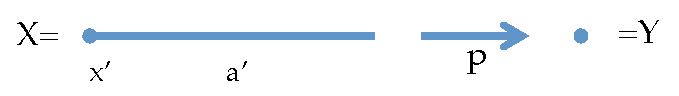
\includegraphics[width=.7\textwidth]{shv_fun_ex1p.pdf}
\caption{Projection to a Point}
\label{fig:shv_fun_ex1}
\end{figure}

Without too much effort we compute the following:
\begin{itemize}
 \item $p_*F=\varprojlim\{F(x')\to F(a')\}\cong F(x')$
 \item $p_{\dd}=\varinjlim\{F(x')\to F(a')\}\cong F(a')$
\end{itemize}

For the pushforward with compact supports, we will be extra careful. Recall the definition states that $p_!F(\tau)=\{s\in\Gamma(p^{-1}(\tau);F)|s(\sigma)=0\, \mathrm{if}\, |\bar{\sigma}|\cap p^{-1}(y)\,\mathrm{not}\,\mathrm{compact}\,\mathrm{for}\, y\in|\tau|\}$.

In our example $y$ can be the only point $\star$ and $p^{-1}(\star)=X$. Thus we have only two cells to check whether their closures are compact or not. Clearly $\bar{x}'=x'$ is compact, but $\bar{a}'=X$ is not compact. The definition then says that we only allow sections whose value on $a'$ is zero.
\begin{itemize}
 \item $p_!F=\ker (\rho_{x',a'}:F(x')\to F(a'))$
\end{itemize}


\subsection{Inclusion into a Closed Interval}\index{cellular maps!inclusion of a point}
Here we encounter an open inclusion $j:X\to Y$. The first thing to note is that in this case, the value of $j_!F$ is not going to change since either $j^{-1}(y)=\{x\}$ or it is empty. Since points are closed and bounded, the compactness condition on $|\bar{\sigma}|\cap \{j^{-1}(y)\}$ is always satisfied.

\begin{figure}[!ht]
\centering
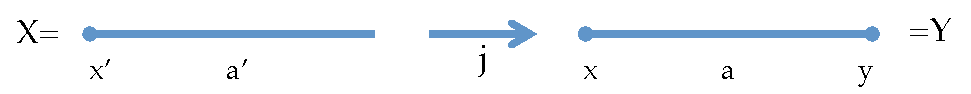
\includegraphics[width=\textwidth]{shv_fun_ex2p.pdf}
\caption{Inclusion into a Closed Interval}
\label{fig:shv_fun_ex2}
\end{figure}

We see in this example that
\begin{itemize}
 \item $j_*F(x)=\varprojlim\{F(x')\to F(a')\}\cong F(x')$, $j_*F(a)=F(a')$, and less intuitively, $j_*F(y)\cong F(a')$.
 \item $j_{\dd}F(x)= F(x')$, $j_{\dd}F(a)\cong F(a')$, and $j_{\dd}F(y)=\varinjlim\{\emptyset\}=0$.
 \item $j_!F\cong j_{\dd}F$.
\end{itemize}


\subsection{Map to a Circle}\index{cellular maps!bijection with a circle}
Here is an example where the function is bijective and continuous (in both topologies), but not an embedding, i.e. the domain is not homeomorphic with its image.

\begin{figure}[h!]
\centering
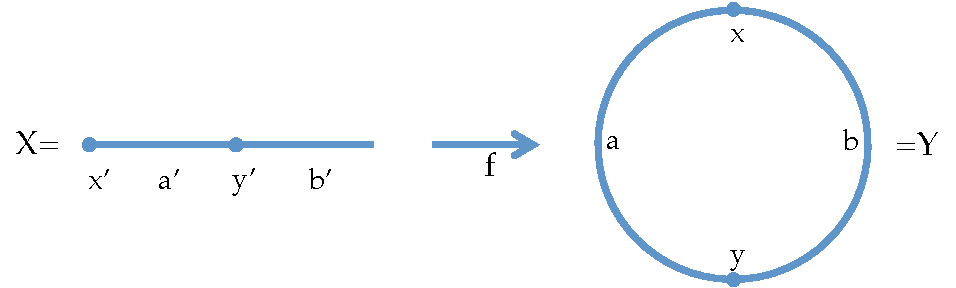
\includegraphics[width=\textwidth]{shv_fun_ex3p.pdf}
\caption{Map to a Circle}
\label{fig:shv_fun_ex3}
\end{figure}

All three sheaves agree on the values and the restriction maps $f_{\Box}F(y)\cong F(y')\to F(a')\cong f_{\Box}F(a)$. We concentrate on the other two cells.
\begin{itemize}
 \item Here diagram we are taking the limit over is disconnected because the inverse image of the star of $x$ in $Y$ is disconnected. Consequently, $f_*F(x)=\varprojlim\{F(x')\to F(a') \quad F(b')\}\cong F(x')\oplus F(b')$ and $f_*F(b)=F(b')$.
 \item Here $f_{\dd}F(x)=F(x')$, but for similar reasons as before $f_{\dd}F(b)=\varinjlim\{F(x')\quad F(y')\to F(b')\}=F(x')\oplus F(b')$.
 \item As noted, $f$ is injective thus the value of $f_!F$ on any cell in the image is un-changed. However, we need to pay careful attention to how the restriction map is defined. The map $f$ is injective so the fiber over $a$ is $a'$ and over $x$ is $x'$, but $x'\nleq a'$ so the restriction map must be zero.
\end{itemize}

\section{The Push-Pull Adjunctions}\label{subsec:adjunctions}
\index{sheaf!push-pull adjunctions}\index{cosheaf!push-pull adjunctions}

Recall from Section~\ref{sec:adjunctions} that adjunctions allow us transform a complicated problem into an easy one. To derive these adjunctions, we can take two approaches: Use Freyd's adjoint functor theorem~\ref{thm:freyd}, or explicitly construct the adjunction. Since in our construction of the functors associated to a map, we made explicit use of limits and colimits, corresponding to the right and left Kan extensions respectively, and (co)limits commute with (co)limits, the following theorems are automatic. However, we check them explicitly for sheaves and leave the dual proof for the reader to fill out on their own.

\begin{thm}
The functors $f^*:\Shv(Y)\to \Shv(X)$ and $f_*:\Shv(X)\to\Shv(Y)$ form an adjoint pair $(f^*,f_*)$ and thus
\[
\Hom_{\Shv(X)}(f^*G,F)\cong \Hom_{\Shv(Y)}(G,f_*F).
\]
Dually, the functors for cosheaves satisfy the opposite adjunction $(f_*,f^*)$
\[
\Hom_{\Coshv(Y)}(f_*\hF,\hG) \cong \Hom_{\Coshv(X)}(\hF,f^*\hG).
\]
\end{thm}
\begin{proof}
	Recall that $f^*(f_*F)(x)=(f_*F)(f(x))$. Using the fact that $(f_*F)(f(x))=\varprojlim\{F(z)|f(z)\geq f(x)\}$, we get a map to $F(x)$ since $x\in f^{-1}(f(x))$ and this morphism is final for each $x$. This implies there is a natural transformation of functors $f^*\circ f_*\to\id$, which is universal (final). 
	
	Similarly, $f_*(f^*G)(y)=\varprojlim\{f^*G(x)=G(f(x))|f(x)\geq y\}$ and since $y\leq f(x)$ we can use the restriction map $\rho^G_{f(x),y}:G(y)\to G(f(x))$. The universal property of the limit guarantees a map $G(y)\to\varprojlim G(f(x))=f_*f^*G(y)$ and thus a natural transformation of functors $\id\to f_*f^*$.
\end{proof}

\begin{thm}
	The functors $f_{\dd}:\Shv(X)\to\Shv(Y)$ and $f^*:\Shv(Y)\to\Shv(X)$ form an adjoint pair $(f_{\dd},f^*)$ and thus
	\[
	\Hom_{\Shv(Y)}(f_{\dd}F,G)\cong\Hom_{\Shv(X)}(F,f^*G).
	\]
	Dually, the functors for cosheaves satisfy the opposite adjunction $(f^*,f_{\dd})$
	\[
	\Hom_{\Coshv(X)}(f^*\hG,\hF) \cong \Hom_{\Coshv(Y)}(\hG,f_{\dd}\hG).
	\]
\end{thm}
\begin{proof}
	$f_{\dd}(f^*G)(y)=\varinjlim \{G(f(x))|f(x)\leq y\}$ so again we can use the restriction maps to define maps to $G(y)$. The universal property of colimits gives a map $f_{\dd}f^*G(y)\to G(y)$ and thus a map of functors $f_{\dd}f^*\to\id$. Similar arguments give a map $\id\to f^*f_{\dd}$
\end{proof}

To conclude, we derive the first interesting consequence of an adjunction. In effect it reduces all the possible natural transformations between a certain pair of functors to a single vector space.
\begin{prop}
	If $F:X\to\Vect$ is a sheaf and $p:X\to\star$ is the constant map, then
	\[
		\Hom_{\Shv(X)}(p^*k,F)\cong \Hom_{\Vect}(k,p_*F)\cong F(X) = H^0(X;F).
	\]
\end{prop}
\begin{proof}
	The first isomorphism is the adjunction $(p^*,p_*)$. The second isomorphism is simply the observation that every linear map is determined by where it sends 1, i.e. $\Hom_{\Vect}(k,W)\cong W$.
\end{proof}
